\documentclass[conference]{IEEEtran}

\usepackage{amsmath,amssymb}
\usepackage{booktabs}
\usepackage{graphicx}
\usepackage{siunitx}
\usepackage{url}
\usepackage[hidelinks]{hyperref}

\graphicspath{{../generated/}}
\sisetup{detect-all,round-mode=places,round-precision=4}

\title{From Offline Optimality to Real-Time Simulation Flight:\
Delay-Aware LQR and Constrained DeePC for an EHEKATL Blended-Wing-Body Aircraft}

\author{%
\IEEEauthorblockN{Author Name(s)}
\IEEEauthorblockA{Department and Institution\\
City, Country\\
email@example.com}}

\begin{document}
\maketitle

\begin{abstract}
Nominal optimal-control results can degrade substantially when transferred to a
high-fidelity flight simulator containing unmodeled actuator routing, hidden
augmentation, input delay, constraints, and operating-point variability. This
paper documents the development of linear-quadratic regulation (LQR) and
regularized constrained data-enabled predictive control (DeePC) for roll-rate
regulation of the EHEKATL blended-wing-body aircraft in X-Plane~12. A
recovery-capable backstepping controller was retained as the stabilizing
baseline and permanent fallback. Stabilized multisine experiments exposed a
measured \SI{35}{\hertz} cascade from commanded yoke input through total control and
distributed surface motion to body roll rate. A delay-aware discrete LQR and a
$P$-only DeePC controller were frozen under identical command and slew limits.
The LQR integrated safely, but its matched-flight integral metric was 0.8888 of
the backstepping result, corresponding to an 11.1\% improvement and failing the
predeclared 30\% target. DeePC passed 243/243 frozen-model uncertainty cases
with worst and median DeePC-to-LQR integral ratios of 0.8953 and 0.7881. In
direct X-Plane demonstrations, both controllers ran at \SI{35}{\hertz}, remained
within constraints, produced measurable recovered responses, and restored
actuator ownership without safety events. DeePC's maximum observed optimization
time was \SI{7.90}{\milli\second} against a \SI{28.57}{\milli\second} control period. Prospective
power analysis nevertheless showed that a defensible superiority experiment
would require 48 pulses per controller for separate reloads, or 24 paired
pulses with an unvalidated switching protocol. The results support safe
real-time implementation and expose the offline-to-simulation gap, but do not
establish DeePC superiority.
\end{abstract}

\begin{IEEEkeywords}
blended-wing body, LQR, DeePC, X-Plane, system identification, real-time
control, flight simulation, safety supervision
\end{IEEEkeywords}

\section{Introduction}
Linear-quadratic regulation provides a transparent state-feedback law and an
explicit state-versus-control tradeoff \cite{kalman1960}. Its practical
conclusions nevertheless depend on model fidelity, state selection, actuator
representation, delay, and operating condition. Data-enabled predictive
control offers a complementary approach: rather than first reducing measured
behavior to a low-order parametric plant, DeePC uses input-output trajectories
to predict and optimize future behavior subject to constraints
\cite{coulson2019,coulson2022}.

The EHEKATL aircraft is a scale blended-wing-body (BWB) model represented in
X-Plane~12. Initial thesis-derived linear time-invariant (LTI) studies produced
stable LQR behavior offline, but direct transfer to X-Plane was unsuccessful.
A historical fixed-gain flight reached \SI{53.0}{\degree} absolute pitch and
\SI{111.9}{\degree} absolute roll, while a second flight repeatedly activated
divergence guards. These failures motivated a stage-gated redevelopment based
on measured actuator realization, independent training and validation data,
immutable performance thresholds, and a recovery-capable backstepping
baseline.

This paper makes four bounded contributions:
\begin{enumerate}
    \item it documents the implementation gap between nominal LQR analysis and
    the realized X-Plane control path;
    \item it presents a stabilized identification procedure and directly
    discrete \SI{35}{\hertz} roll cascade;
    \item it implements constrained LQR and DeePC behind a common safety,
    fallback, and actuator-restoration contract; and
    \item it reports successful real-time integration together with failed
    performance and power gates without retrospectively weakening them.
\end{enumerate}
The experiments are real-time closed-loop simulation flights, not
physical-aircraft flight tests.

\section{Aircraft and Experimental Environment}
The test article was the EHEKATL BWB G33 scale aircraft in X-Plane~12.4.3-r2,
interfaced through the NASA XPlaneConnect architecture \cite{nasaXPC}. The
frozen local operating condition, denoted R3, is summarized in
Table~\ref{tab:condition}. Manual/Clear weather, no declared failures, enabled
X-Plane artificial stability, disabled autopilot and autothrottle, live
simulation speed, and replay off were required.

\begin{table}[t]
\caption{Frozen R3 Operating Condition and Limits}
\label{tab:condition}
\centering
\begin{tabular}{@{}ll@{}}
\toprule
Quantity & Value \\
\midrule
Altitude & approximately \SI{1700}{\metre} \\
Indicated airspeed & approximately \SI{39}{\knot} \\
Dynamic pressure & approximately \SI{240}{\pascal} \\
Pitch / roll & \SI{1.3}{\degree} / near \SI{0}{\degree} \\
Cockpit throttle & 0.02353 \\
Primary output & body roll rate $P$ \\
Control frequency & \SI{35}{\hertz} \\
Command bound & 0.0002 normalized \\
Slew bound & 0.00005 per sample \\
Fallback update rate & \SI{10}{\hertz} \\
Safety envelope & $|\phi|,|\theta|\leq\SI{10}{\degree}$; \\
 & $|P|,|Q|,|R|\leq\SI{20}{\degree\per\second}$ \\
\bottomrule
\end{tabular}
\end{table}

The common manipulated variable was trim-relative yoke-roll perturbation. Body
roll rate $P$ was the primary regulated output. Roll angle, total roll-control
ratio, distributed aileron deflection, moments, simulator state, override
ownership, and timing were retained as audit channels. Both optimized
controllers ran at \SI{35}{\hertz}. The original backstepping law was updated at its
validated \SI{10}{\hertz} rate and held between updates when serving as fallback.

\section{Control-Path Diagnosis and Identification}
Early experiments showed that a transmitted XPlaneConnect CTRL packet did not
necessarily equal the realized actuator input. When the simulator was paused or
in replay, writable yoke values could change without advancing surfaces or
aircraft dynamics. Even in live simulation, physical joystick input could
overwrite nonpersistent commands between controller updates. Persistent
per-axis ownership and direct yoke writes were therefore required.

Taking ownership exposed an additional trim problem. The original controller
implicitly relied on a physical pitch input near 0.149 normalized units. A
first owned-axis handoff removed this contribution and produced a pitch-rate
transient of approximately \SI{-13.85}{\degree\per\second}. Subsequent tests captured the
realized trim before ownership and applied controller outputs as trim-relative
perturbations. Artificial stability remained active and altered the mapping
between yoke command and total control; measured total control, rather than sent
command alone, was therefore used for plant identification.

Stabilized multisine experiments were superimposed on backstepping instead of
replacing it. Two training and two held-out validation runs were collected for
each of roll and pitch. All eight datasets passed completeness, realization,
spectral-richness, safety, and restoration gates. A \SI{10}{\hertz} local angle/rate
model identified a three-sample input delay but retained colored residuals.
Higher-rate testing subsequently isolated the cascade
\begin{equation}
u_{y,k}\longrightarrow u_{t,k}\longrightarrow \delta_{a,k}
\longrightarrow P_k,
\label{eq:cascade}
\end{equation}
where commanded yoke perturbation maps dynamically to total roll control,
total control maps nearly statically to distributed aileron motion, and surface
motion maps dynamically to roll rate. Temporal held-out validation supported a
directly discrete \SI{35}{\hertz} cascade. Continuous-time pole interpretations were
rejected because their fitted time constants were at or below the sampling
interval.

\section{Controller Design}
\subsection{Delay-Aware LQR}
The frozen roll-rate LQR state was
\begin{equation}
x_k=[\Delta P_k,\ \Delta u_{t,k},\ \Delta u_{y,k-1}]^T,
\end{equation}
with dynamics $x_{k+1}=Ax_k+Bu_k$, where
\begin{equation}
A=\begin{bmatrix}
0.40856&3.55738&37.94551\\
0&0.05609&0.59835\\
0&0&0
\end{bmatrix},\quad
B=\begin{bmatrix}23.90120\\0.37689\\1\end{bmatrix}.
\end{equation}
The infinite-horizon quadratic objective was
\begin{equation}
J=\sum_{k=0}^{\infty}\left(x_k^TQx_k+u_k^TRu_k\right),
\end{equation}
subject at runtime to the common command and slew limits. The resulting gain
was
\begin{equation}
K=[0.0002944,\ 0.0027424,\ 0.0292528].
\end{equation}
The nominal closed-loop spectral radius was 0.3684. Across 243 coefficient
combinations, the worst spectral radius was 0.4936 with no unstable cases.
These values establish robustness of the frozen measured-cascade model, not
global stability of the X-Plane aircraft.

\subsection{Regularized Constrained DeePC}
The selected DeePC used one input (trim-relative yoke-roll perturbation) and one
output (roll-rate perturbation). Attempts to predict $P$, roll angle, and total
roll control jointly failed the reconstruction gate, so the final claim is
explicitly $P$-only. Hankel matrices were constructed from a frozen design
trajectory following the behavioral parameterization in
\cite{willems2005,coulson2019}. Each update solved a regularized finite-horizon
problem of the form
\begin{equation}
\min_g\ \|y_f\|_{Q_y}^2+\|u_f\|_{R_u}^2+
\|\Delta u_f\|_{R_{\Delta u}}^2+\lambda_g\|g\|_2^2,
\label{eq:deepc}
\end{equation}
subject to past input/output consistency, future behavioral constraints, and
hard command/slew bounds. Table~\ref{tab:controllers} records the frozen
parameters.

\begin{table}[t]
\caption{Frozen Controller Parameters}
\label{tab:controllers}
\centering
\begin{tabular}{@{}lll@{}}
\toprule
Parameter & LQR & DeePC \\
\midrule
Sample rate & \SI{35}{\hertz} & \SI{35}{\hertz} \\
Primary output & $P$ & $P$ \\
State/history & 3 states & $T_{\mathrm{ini}}=5$ \\
Prediction horizon & infinite & 5 samples \\
$Q_y$ / $R_u$ & --- & 1 / 0.01 \\
$R_{\Delta u}$ & --- & 0.02 \\
$\lambda_g$ & --- & 10 \\
Command bound & 0.0002 & 0.0002 \\
Slew bound & 0.00005 & 0.00005 \\
\bottomrule
\end{tabular}
\end{table}

Constant DeePC optimizer matrices were precomputed, reducing online runtime
without changing controller output; packaged-versus-design command error was
exactly zero. The runtime contained a permanent fallback latch. Nonfinite
inputs, optimizer nonconvergence, deadline violation, simulator-state
violation, or safety-envelope violation permanently transferred command
selection to bounded backstepping. Automatic DeePC re-engagement was prohibited.

\section{Experimental Protocol and Metrics}
Every engaged run first evaluated altitude, airspeed, pitch, roll, body rates,
artificial-stability state, override ownership, pause, simulation speed, and
replay mode. A failed start gate sent no control. After a passing gate, roll and
pitch axes were owned explicitly. Pitch remained stabilized by the original
backstepping law, while the tested controller supplied roll perturbation.
Captured yoke values were restored in an unconditional cleanup path and
verified after the run.

The primary performance measure was time-integrated absolute roll-rate
deviation. Secondary measures included peak and final-window roll-rate
deviation, control energy, command and slew utilization, computation time,
deadline misses, fallback events, and restoration error. Performance thresholds
and dataset roles were frozen before confirmation data were opened. A safe run
was treated as integration evidence, not automatically as a performance pass.

\section{Results}
\subsection{LQR Matched-Performance Result}
The measured-cascade LQR passed its integration and safety prerequisites. In
the frozen matched backstepping/LQR flight pair, the final integral ratio was
0.888807, an 11.1\% reduction relative to backstepping. The predeclared gate
required a ratio no greater than 0.70, so the LQR performance claim failed. The
ratio worsened as the quiet tail was accumulated, indicating that
reload-specific background motion dominated the small disturbance response.

\subsection{DeePC Offline Robustness and Integration}
The final DeePC candidate converged in all 243 frozen-model uncertainty cases.
The worst and median DeePC/LQR integral ratios were 0.895344 and 0.788056, and
the worst peak ratio was 0.928154. Maximum command and base slew were
$4.39\times10^{-5}$ and $9.97\times10^{-6}$, respectively. A guarded design
pilot passed all integration gates and was excluded from confirmation.

\subsection{Direct Demonstrations}
Table~\ref{tab:direct} reports two user-requested direct demonstrations. Each
began after a fresh R3 reload; the values are descriptive, not a matched
comparison. Both flights completed 1050 samples without fallback, saturation,
safety events, or restoration errors.

\begin{table*}[t]
\caption{Direct R3 Demonstrations From Separate Reloads}
\label{tab:direct}
\centering
\begin{tabular}{@{}lrrrrrrrr@{}}
\toprule
Controller & Rate & Max gap & IAE & RMS $|\Delta P|$ & Peak $|\Delta P|$ & Final max & Peak cmd. & Max slew \\
 & (Hz) & (ms) & (deg) & (deg/s) & (deg/s) & (deg/s) & & \\
\midrule
DeePC & 35.0014 & 50.09 & 0.01972 & 0.000796 & 0.004163 & 0.001311 & $4.609\!\times\!10^{-5}$ & $2.126\!\times\!10^{-5}$ \\
LQR   & 35.0040 & 42.23 & 0.02025 & 0.000863 & 0.005622 & 0.001496 & $4.670\!\times\!10^{-5}$ & $2.171\!\times\!10^{-5}$ \\
\bottomrule
\end{tabular}
\end{table*}

DeePC median, 95th-percentile, and maximum optimization times were 4.02, 5.36,
and \SI{7.90}{\milli\second}, respectively, below the \SI{28.57}{\milli\second} sample period. Both
controller runtimes reproduced their frozen offline behavior exactly. The
slightly smaller DeePC response metrics cannot be interpreted causally because
the initial reloads and background trajectories were not matched.

\begin{figure*}[t]
\centering
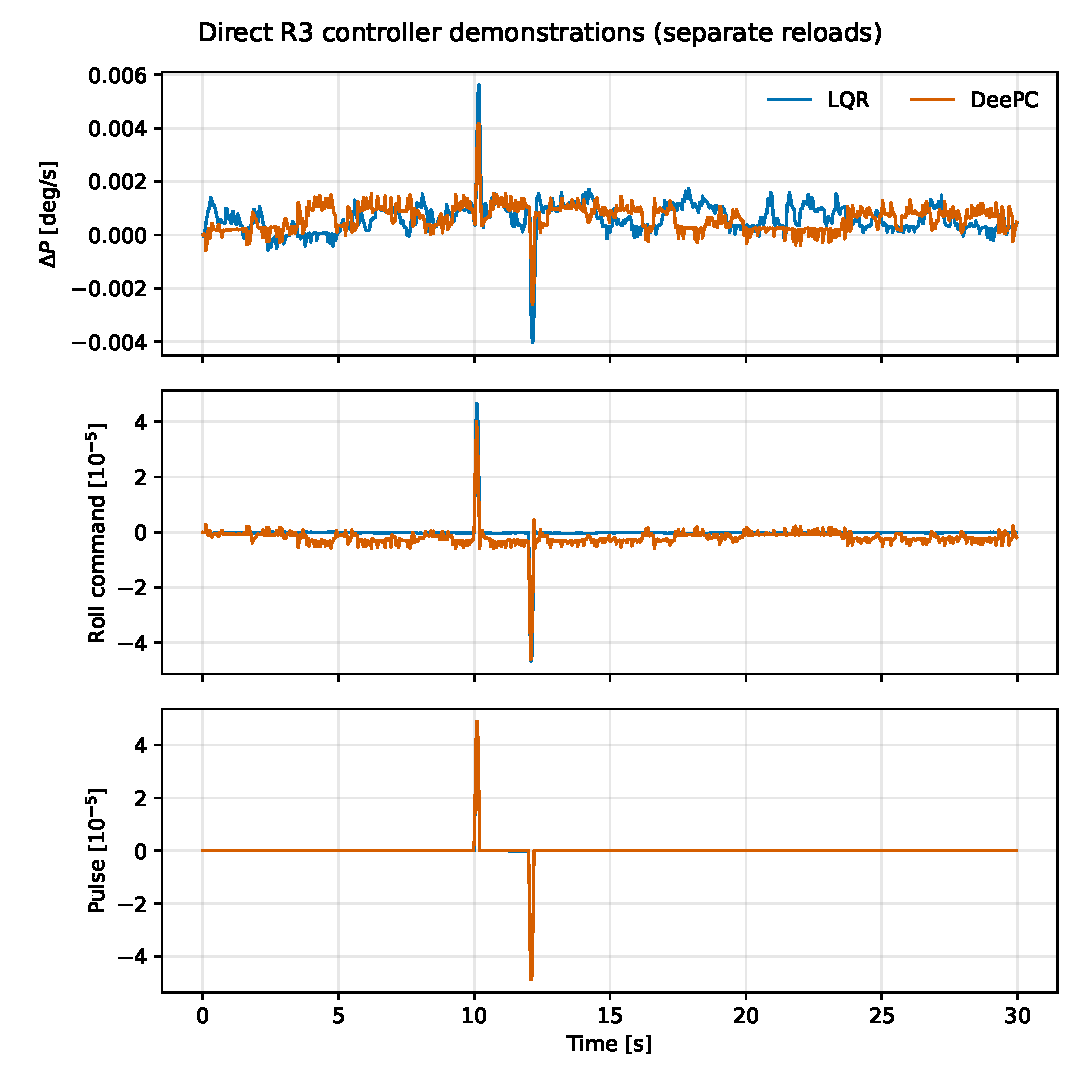
\includegraphics[width=0.88\textwidth]{direct_controller_demonstrations.pdf}
\caption{Direct LQR and DeePC demonstrations at R3. Curves are overlaid for
descriptive inspection only; the controllers were tested after separate
reloads, so the plot is not a matched superiority comparison.}
\label{fig:direct}
\end{figure*}

\subsection{Prospective Power}
Prospective moving-block bootstrap analyses quantified the cost of an
independent superiority claim. A separate-reload design first exceeded 0.80
power at 48 pulses per controller, requiring at least \SI{149}{\second} per
controller. A paired mean per-pulse IAE design achieved power 0.7967 at 16
pairs, which failed the unchanged 0.80 gate; it first qualified at 24 pairs and
at least \SI{152}{\second}. That design also required controller switching and
history handoffs not validated in flight. The benchmark was therefore rejected
before collection.

\begin{figure*}[t]
\centering
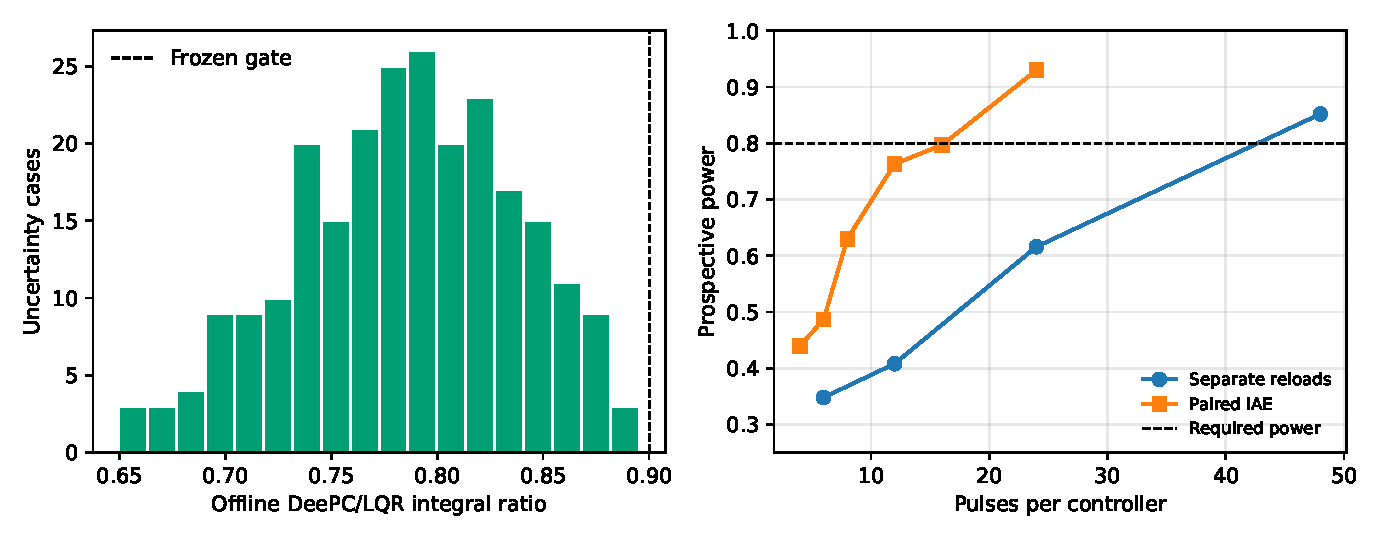
\includegraphics[width=0.88\textwidth]{offline_robustness_and_power.pdf}
\caption{Left: frozen-model DeePC/LQR integral ratios over 243 uncertainty
cases. Right: prospective statistical power versus pulse count. The apparent
offline advantage was too small relative to reload variability for a practical
confirmation campaign.}
\label{fig:power}
\end{figure*}

\section{Discussion}
The experiments show why offline optimality and online performance must be
treated separately. The LQR was stable and robust over its identified model,
yet its matched improvement was small in X-Plane. The dominant complications
were not Riccati-solver limitations: they were control ownership, hidden trim,
artificial-stability dynamics, a dynamic commanded-to-realized input path,
local model validity, and reload-specific background motion.

DeePC reduced dependence on an explicit low-order state realization and passed
the frozen offline robustness gate. It also met the real-time computational
budget comfortably. Using measured data, however, does not eliminate
distribution shift. The selected controller predicts only $P$, its design data
come from a local R3 trajectory, and the effect expected over LQR was too small
relative to observed variability for an economical confirmation campaign.

The negative gates are an engineering result. Relaxing the 30\% LQR target
after observing an 11.1\% improvement, rounding 0.7967 power to 0.80, or
presenting separate-reload demonstrations as a matched comparison would each
overstate the evidence. Preserving these failures yields a reproducible account
of what the controllers do reliably: bounded local roll-rate regulation with
verified real-time execution, fallback readiness, and actuator restoration.

\section{Limitations}
The conclusions apply only near R3 and do not establish transfer to other
airspeeds, dynamic pressures, mass properties, weather conditions, or failure
states. Artificial stability was enabled and forms part of the tested plant.
The work validates roll-rate behavior, not a complete attitude loop, combined
longitudinal/lateral operation, or large-disturbance recovery. DeePC is
$P$-only, and the direct demonstrations are single unmatched flights. Finally,
X-Plane is a high-fidelity simulation environment, not physical flight
hardware; network, sensor, actuator, and aerodynamic effects on a real aircraft
may differ.

\section{Conclusion}
A delay-aware measured-cascade LQR and a regularized constrained DeePC were
implemented successfully for the EHEKATL BWB in real-time X-Plane flight. Both
direct demonstrations met timing, command, slew, safety, exact-replay,
fallback, and actuator-restoration requirements. DeePC optimization remained
well within the \SI{35}{\hertz} deadline. However, LQR failed its predeclared 30\%
matched-improvement gate, and a powered DeePC-versus-LQR superiority experiment
was impractical under the available local protocol. The appropriate conclusion
is not that one controller universally outperforms the other, but that safe
implementation is achievable while predicted performance differences can be
overwhelmed by the realized control path and operating variability. Future work
should prioritize multi-regime data, state/augmentation measurements,
gain-scheduled or multi-dataset formulations, and a prospectively powered
common benchmark before extending to attitude control.

\section*{Data and Reproducibility}
Every paper-facing dataset is listed with its role and SHA256 hash in the
project dataset registry. Raw logs, frozen numerical artifacts, controller
code, and analysis code are retained separately. All tables and figures in this
paper are generated by a deterministic paper-facing analysis script. Design,
demonstration, and held-out evidence remain distinct; no physical-aircraft data
are claimed.

\begin{thebibliography}{00}
\bibitem{kalman1960}
R. E. Kalman, ``Contributions to the theory of optimal control,'' \emph{Boletín
de la Sociedad Matemática Mexicana}, vol. 5, pp. 102--119, 1960.

\bibitem{coulson2019}
J. Coulson, J. Lygeros, and F. Dörfler, ``Data-enabled predictive control: In
the shallows of the DeePC,'' in \emph{Proc. European Control Conf.}, 2019,
pp. 307--312, doi: 10.23919/ECC.2019.8795639.

\bibitem{coulson2022}
J. Coulson, J. Lygeros, and F. Dörfler, ``Distributionally robust chance
constrained data-enabled predictive control,'' \emph{IEEE Trans. Autom.
Control}, vol. 67, no. 7, pp. 3289--3304, 2022,
doi: 10.1109/TAC.2021.3097706.

\bibitem{willems2005}
J. C. Willems, P. Rapisarda, I. Markovsky, and B. L. M. De Moor, ``A note on
persistency of excitation,'' \emph{Syst. Control Lett.}, vol. 54, no. 4,
pp. 325--329, 2005, doi: 10.1016/j.sysconle.2004.09.003.

\bibitem{nasaXPC}
NASA Ames Research Center, ``X-Plane Communication Toolbox (XPC),'' NASA
Software Catalog, ARC-17185-1. [Online]. Available:
\url{https://software.nasa.gov/software/ARC-17185-1}. Accessed: Aug. 10, 2026.
\end{thebibliography}

\end{document}
